% Hlavicka pro protokoly z fyzikalniho praktika.
% Verze pro: LaTeX
% Verze hlavicky: 22. 2. 2007
% Autor: Ustav fyziky kondenzovanych latek
% Ke stazeni: www.physics.muni.cz/ufkl/Vyuka/
% Licence: volne k pouziti, nejlepe k vcasnemu odevzdani protokolu z Vaseho mereni.

\documentclass[a4paper,11pt]{article}

% Kodovani (cestiny) v dokumentu: utf-8
%\usepackage[cp1250]{inputenc}	% Omezena stredoevropska kodova stranka, pouze MSW.
\usepackage[utf8]{inputenc}	% Doporucujeme pouzivat UTF-8 (unicode).
\usepackage[T1]{fontenc}
\usepackage{lmodern}

%%% Nemente:
\usepackage[margin=2cm]{geometry}
\newtoks\jmenopraktika \newtoks\jmeno \newtoks\datum
\newtoks\obor \newtoks\skupina \newtoks\rocnik \newtoks\semestr
\newtoks\cisloulohy \newtoks\jmenoulohy
\newtoks\tlak \newtoks\teplota \newtoks\vlhkost
\usepackage{amsmath}
\usepackage{mathtools}
\usepackage{graphicx}
\usepackage{multirow}

\usepackage{pgfplotstable} 
\usepackage{booktabs}

\graphicspath{ {./images/} }
%%% Nemente - konec.


%%%%%%%%%%% Doplnte pozadovane polozky:

\jmenopraktika={Fyzikální praktikum 3}  % nahradte jmenem vaseho predmetu
\jmeno={Artem Gorodilov}            % nahradte jmenem mericiho
\datum={6. ~května  2024}        % nahradte datem mereni ulohy
\obor={Astrofyzika}                     % nahradte zkratkou vami studovaneho oboru
\skupina={Po 14:00}            % nahradte dobou vyuky vasi seminarni skupiny
\rocnik={II}                  % nahradte rocnikem, ve kterem studujete
\semestr={II}                 % nahradte semestrem, ve kterem studujete

\cisloulohy={F}               % nahradte cislem merene ulohy
\jmenoulohy={Optická emisní spektra atomů a molekul} % nahradte jmenem merene ulohy

\tlak={979}                   % nahradte tlakem pri mereni (v hPa)
\teplota={21.4}               % nahradte teplotou pri mereni (ve stupnich Celsia)
\vlhkost={46}               % nahradte vlhkosti vzduchu pri mereni (v %)

%%%%%%%%%%% Konec pozadovanych polozek.


%%%%%%%%%%% Uzitecne balicky:
\usepackage[czech]{babel}
\usepackage{graphicx}
\usepackage{amsmath}
\usepackage{xspace}
\usepackage{url}
\usepackage{indentfirst}
\usepackage{listings}
\usepackage{subcaption}
\usepackage{caption}
\usepackage{tabularx}
\usepackage[labelformat=parens,labelsep=quad,skip=3pt]{caption}

%%%%%% Zamezeni parchantu:
\widowpenalty 10000 \clubpenalty 10000 \displaywidowpenalty 10000
%%%%%% Parametry pro moznost vsazeni vetsiho poctu obrazku na stranku
\setcounter{topnumber}{3}	  % max. pocet floatu nahore (specifikace t)
\setcounter{bottomnumber}{3}	  % max. pocet floatu dole (specifikace b)
\setcounter{totalnumber}{6}	  % max. pocet floatu na strance celkem
\renewcommand\topfraction{0.9}	  % max podil stranky pro floaty nahore
\renewcommand\bottomfraction{0.9} % max podil stranky pro floaty dole
\renewcommand\textfraction{0.1}	  % min podil stranky, ktery musi obsahovat text
\intextsep=8mm \textfloatsep=8mm  %\intextsep pro ulozeni [h] floatu a \textfloatsep pro [b] or [t]

% Tecky za cisly sekci:
\renewcommand{\thesection}{\arabic{section}.}
\renewcommand{\thesubsection}{\thesection\arabic{subsection}.}
% Jednopismenna mezera mezi cislem a nazvem kapitoly:
\makeatletter \def\@seccntformat#1{\csname the#1\endcsname\hspace{1ex}} \makeatother

\begin{document}

\thispagestyle{empty}

{
\begin{center}
\sf 
{\Large Ústav fyzikální elektroniky PřF MU} \\
\bigskip
{\huge \bfseries FYZIKÁLNÍ PRAKTIKUM} \\
\bigskip
{\Large \the\jmenopraktika}
\end{center}

\bigskip

\sf
\noindent
\setlength{\arrayrulewidth}{1pt}
\begin{tabular*}{\textwidth}{@{\extracolsep{\fill}} l l}
\large {\bfseries Zpracoval:}  \the\jmeno & \large  {\bfseries Naměřeno:} \the\datum\\[2mm]
\large  {\bfseries Obor:} \the\obor  \hspace{40mm}  {\bfseries Skupina:} \the\skupina %
%{\bfseries Ročník:} \the\rocnik \hspace{5mm} {\bfseries Semestr:} \the\semestr  
&\large {\bfseries Testováno:}\\
\\
\hline
\end{tabular*}
}

\bigskip

{
\sf
\noindent \begin{tabular}{p{3cm} p{0.6\textwidth}}
\Large  Úloha č. {\bfseries \the\cisloulohy:} \par
\smallskip
% $T=\the\teplota$~$^\circ$C \par
% $p=\the\tlak$~hPa \par
% $\varphi=\the\vlhkost$~\%
&\Large \bfseries \the\jmenoulohy  \\[2mm]
\end{tabular}
}

\vskip10pt
    \begin{minipage}[t]{0.5\textwidth} 
        \section{Zadání}    
            \begin{enumerate}
                \item Identifikovat spektrální čáry emitované parami materiálu elektrod v obloukovém výboji a určit jejich intenzitu. 
                \par Ze sklonu pyrometrické přímky určit teplotu oblouku.
                \item Určit z naměřeného molekulového spektra radikálu OH rotační teplotu.
            \end{enumerate}
        \section{Teorie}
            \subsection{Spektrální čáry}
                \par Spektrální čáry jsou způsobeny přechody elektronů mezi energetickými hladinami atomu nebo molekuly. Energie přechodu je rovna rozdílu energií hladin a odpovídá energii fotonu emitovaného nebo absorbovaného při přechodu. Spektrální čáry jsou charakteristické pro každý prvek a slouží k identifikaci prvků ve vzorcích.
                \par Relativní intenzita spektrálních čar je dána vztahem:
                \begin{equation}
                    I_{mn} \sim \frac{A_{mn}g_m}{\lambda_m} \cdot \exp\left(-\frac{E_{m}}{kT}\right)
                \end{equation}
                kde $A_{mn}$ je pravděpodobnost přechodu s m-té na n-tou hladinu, $g_m$ je statistická váha horního energetického stavu, $\lambda_m$ je vlnová délka emitovaného fotonu, $E_m$ je excitační energie m-té hladiny, $k$ je Boltzmannova konstanta a $T$ je teplota.
                \par Po zalogování vztahu (1) dostaneme:
                \begin{equation}
                    \ln\left(\frac{I_{mn}\lambda_{mn}}{A_{mn}g_m}\right) \sim \left(-\frac{E_{m}}{kT}\right)
                \end{equation}
                \par Závislost intenzity spektrální čáry na teplotě je tedy lineární (tzv. pyrometrická přímka):
    \end{minipage}
    \hspace{10pt}
    \begin{minipage}[t]{0.5\textwidth} 
                \begin{equation}
                    y = \ln\left(\frac{I_{mn}\lambda_{mn}}{A_{mn}g_m}\right) = f(E_m)
                \end{equation}

            \subsection{Molekulové spektrum}
                \par Molekulové spektrum je dáno kvantovými čísly $N$, $J$ a $S$, které popisují rotaci a vibraci molekuly. Intenzita rotační čáry je dána vztahem:
                \begin{equation}
                    \ln \left(\frac{I_{n''v''J''}^{n'v'J'}}{\tilde{\nu}^4 S_{J'J''}}\right) = -\frac{B_{v'}hc}{kT}N'(N'+1) + const
                \end{equation}
                kde $I_{n''v''J''}^{n'v'J'}$ je intenzita spektrální čáry, $\tilde{\nu}$ je vlnočet, $S_{J'J''}$ je Hönl-Londonův intensitní faktor, $B_{v'}$ je rotační konstanta, $N'$ je rotační kvantové číslo, $h$ je Planckova konstanta a $c$ je rychlost světla.

        \section{Měření}   
            \subsection{Spektrá železa}
                Pomocí programu $Span$ \cite{span} jsme určili a zkalibrovali spektrální čáry spektra železa, které jsme dostali, a změřili intenzity těchto čar. Data jsou uvedena v tabulce (1). Spektra jsou znázorněna v grafu (\ref{fig:Fe_spec}).

                \vspace{15pt}   
                \par \centering
                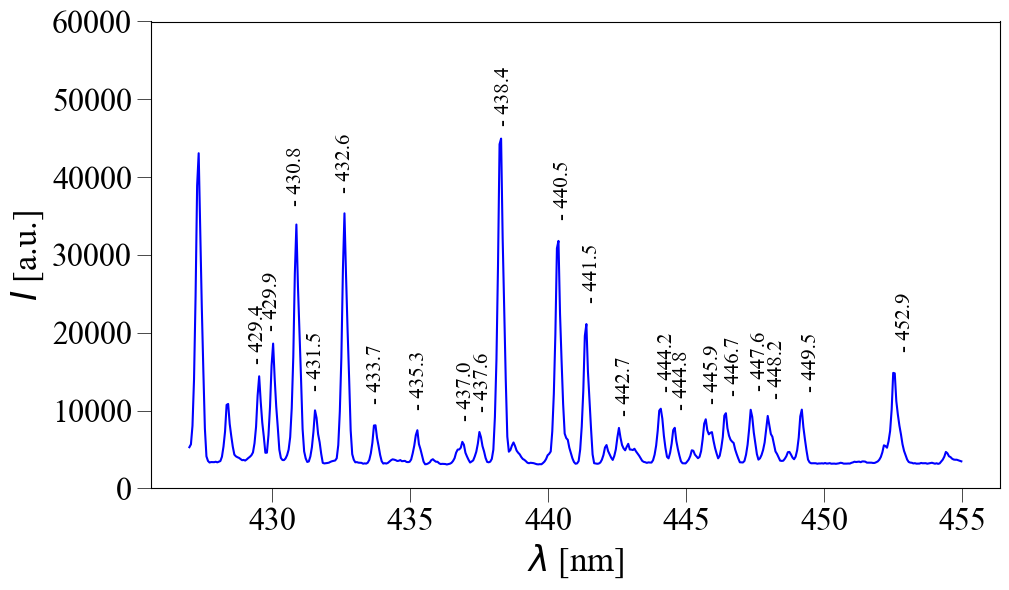
\includegraphics[scale=0.33]{Fe_spec}
                \captionsetup{justification=centering, font=footnotesize}
                \captionof{figure}{Spektrá železa.}
                \label{fig:Fe_spec}
                \vspace{10pt}
                \raggedright   
                
    \end{minipage}
\newpage
    \begin{minipage}[t]{0.5\textwidth} 
                \par Pomocí tohoto programu jsme také provedli pyrometrickou přímku a určili tak teplotu materiálu: 
                \begin{center}
                    $T_{Fe, span}$ = (6371 $\pm$ 934) K
                \end{center}
                Z tabulkových údajů jsme získali hodnoty $A$ a $E$, poté jsme určili teplotu vynesením pyrometrické přímky podle vzorce (3). Výsledky jsou znázorněny v grafu (\ref{fig:Fe}). 
                \begin{center}
                    $T_{Fe}$ = (5600 $\pm$ 400) K
                \end{center}

                \vspace{10pt}   
                \par \centering
                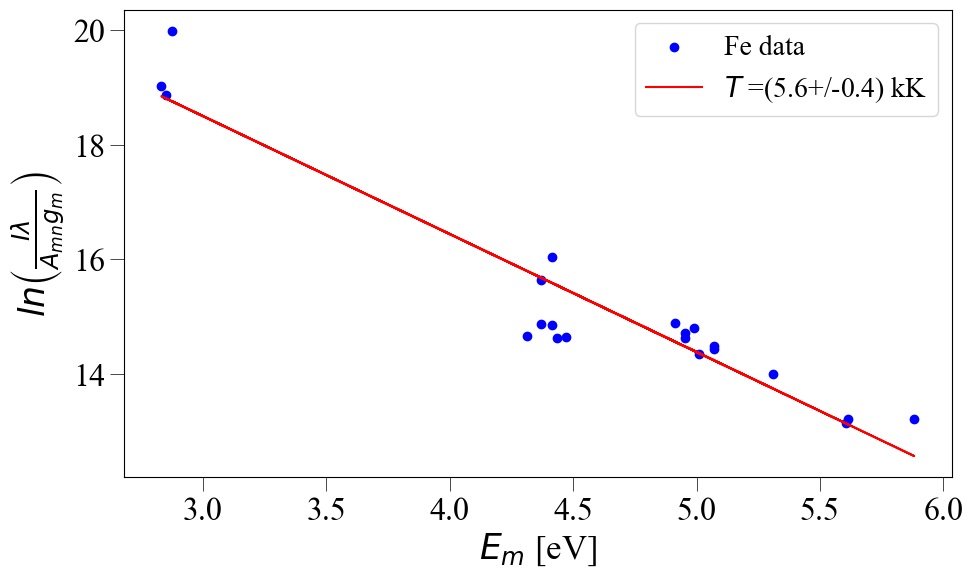
\includegraphics[scale=0.33]{Fe}
                \captionsetup{justification=centering, font=footnotesize}
                \captionof{figure}{Pyrometrická přímka pro železo.}
                \label{fig:Fe}
                \vspace{10pt}
                \raggedright   

            \subsection{Molekulové spektrum radikálu OH}
                Pomocí programu $Span$ jsme určili a zkalibrovali rotační čáry molekulového spektra radikálu OH, které jsme dostali, a změřili intenzity těchto čar. Data jsou uvedena v tabulce (2). Spektra jsou znázorněna v grafu (\ref{fig:OH_spec}).

                \vspace{10pt}   
                \par \centering
                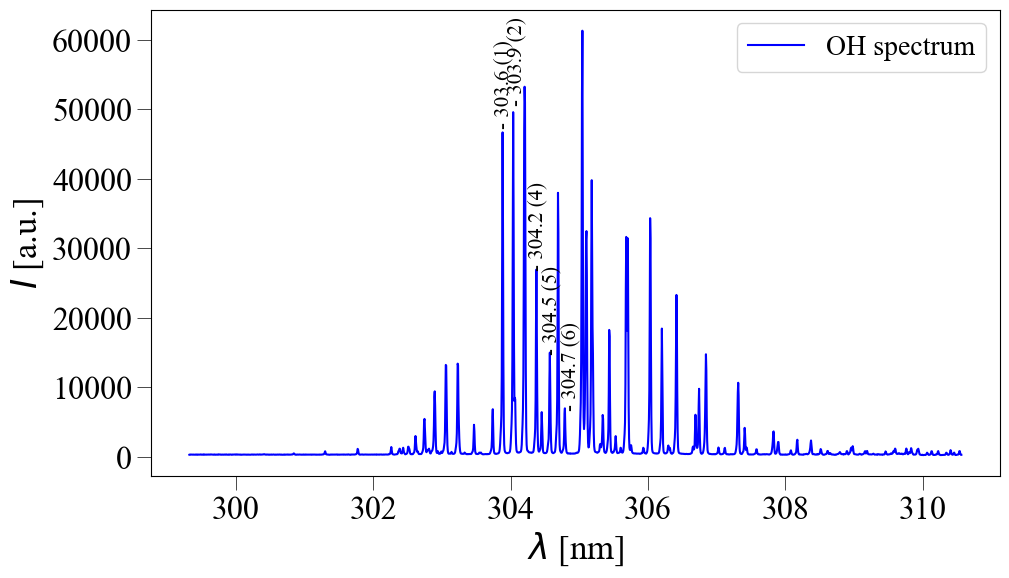
\includegraphics[scale=0.33]{OH_spec}
                \captionsetup{justification=centering, font=footnotesize}
                \captionof{figure}{Rotční spektra radikálu OH. Rotční čárz jsou označeny čísly.}
                \label{fig:OH_spec}
                \vspace{10pt}
                \raggedright  

                \par Pomocí tohoto programu jsme také provedli pyrometrickou přímku a určili tak teplotu materiálu: 
                \begin{center}
                    $T_{OH, span}$ = (302 $\pm$ 11) K
                \end{center}

                Z tabulkových údajů jsme získali hodnoty $S_{J'J''}$ a $J'$, poté jsme určili teplotu vynesením
    \end{minipage}
    \hspace{10pt}
    \begin{minipage}[t]{0.5\textwidth} 
                pyrometrické přímky podle vzorce (4). Výsledky jsou znázorněny v grafu (\ref{fig:OH}):
                \begin{center}
                    $T_{OH}$ = (269 $\pm$ 11) K
                \end{center}

                \vspace{10pt}   
                \par \centering
                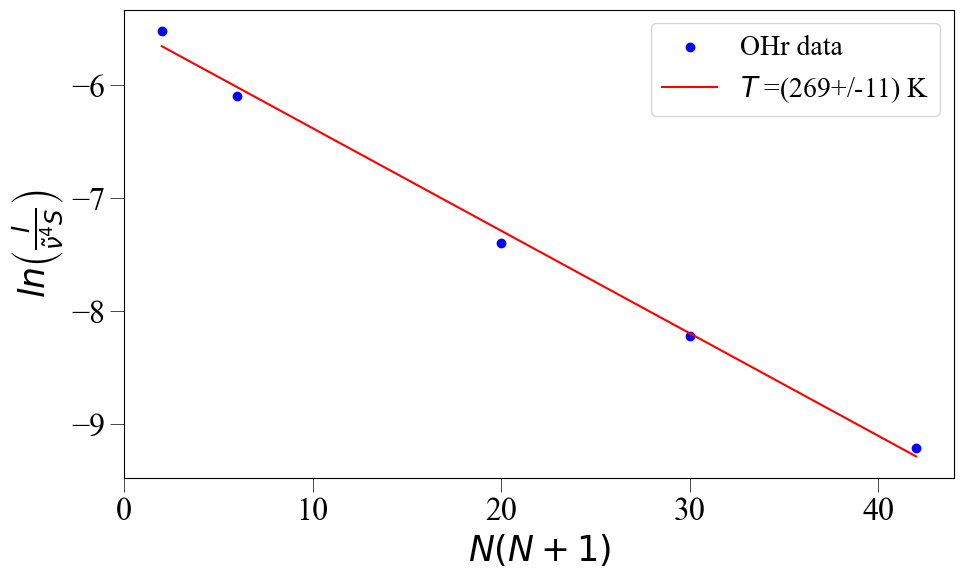
\includegraphics[scale=0.33]{OH}
                \captionsetup{justification=centering, font=footnotesize}
                \captionof{figure}{Pyrometrická přímka pro radikál OH.}
                \label{fig:OH}
                \vspace{10pt}
                \raggedright 

                \vspace{10pt}
                \par K výpočtu veličin a jejich nejistot byla použita knihovna Uncertinties pro Python \cite{uncertainties}. Chyby byly rozšířeny o Studentův koeficient (2-Tail Confidence Level) s ohledem na stupně volnosti pro každou hodnotu, pro interval spolehlivosti 68.27\%.

        \section{Závěr}
                \par Byly identifikovány spektrální čáry emitované parami materiálu elektrod v obloukovém výboji a určeny jejich intenzity. Ze sklonu pyrometrické přímky pro spektrum železa byla určena teplota oblouku: $T_{Fe}$ = (5600 $\pm$ 400) K a pomocí programu $Span$ byla určena teplota: $T_{Fe, span}$ = (6371 $\pm$ 934) K.
                \vspace{10pt}
                \par Byla určena rotační teplota radikálu OH: $T_{OH}$ = (269 $\pm$ 11) K a pomocí programu $Span$ byla určena teplota: $T_{OH, span}$ = (302 $\pm$ 11) K.
                \vspace{10pt}
                \par Získané teploty lze interpretovat různě v závislosti na experimentálních podmínkách. Teplota $T$ získaná z pyrometrické čáry z emisního (rotačního) atomového spektra je obecně emisní nebo excitační teplota \cite{excitation}. Může zastupovat skutečnou kinetickou teplotu \cite{kinetic}, pokud je systém v LTE (Lokální Termodynamická Rovnováha), ale za podmínek mimo LTE slouží jako efektivní teplota $T_{eff}$ \cite{effective} udávající rozložení energie mezi emitujícími druhy.
                \vspace{10pt}
                \par Rozdíl mezi $T_{Fe}$, $T_{Fe, span}$ a $T_{OH}$, $T_{OH, span}$ v obou případech je způsoben kalibrace spektrálních čar a použitím různých spektralních konsant.

                
    \end{minipage}
\newpage
                \renewcommand{\refname}{Odkazy}
                \begin{thebibliography}{9}
                    \bibitem{span}
                        Span, Dostupné online: \url{https://www.physics.muni.cz/~zdenek/span/}
                    \bibitem{uncertainties}
                        Uncertainties, Dostupné online: \url{https://pypi.org/project/uncertainties}
                    \bibitem{excitation}
                        M. P. Polek, M. C. Phillips, F. N. Beg, S. S. Harilal; Comparison of excitation temperature of a laser-produced plasma by combining emission and absorption spectroscopy. AIP Advances 1 February 2024; 14 (2): 025043. doi: \url{https://doi.org/10.1063/5.0190522}
                    \bibitem{kinetic}
                        A. Yanguas-Gil, J. Cotrino, A. R. González-Elipe; Measuring the electron temperature by optical emission spectroscopy in two temperature plasmas at atmospheric pressure: A critical approach. J. Appl. Phys. 1 February 2006; 99 (3): 033104. doi: \url{https://doi.org/10.1063/1.2170416}
                    \bibitem{effective}
                        S. L. Siddanathi, L. G. Westerberg, H. O. Åkerstedt, H. Wiinikka, A. Sepman; Computational modeling and temperature measurements using emission spectroscopy on a non-transferred plasma torch. AIP Advances 1 February 2023; 13 (2): 025019. doi: \url{https://doi.org/10.1063/5.0129653}
                \end{thebibliography} 

    \begin{center}
        \section{Appendix}
            \subsection{Tabulka naměřených hodnot pro spektrální čáry železa}
                \pgfplotstabletypeset[
                col sep=comma, % Defines the separator, comma for CSV
                string type, % Treats columns as strings (not math mode)
                every head row/.style={before row=\toprule,after row=\midrule},
                every last row/.style={after row=\bottomrule},
                columns/lam/.style={column name=$\lambda$ [nm]},
                columns/int/.style={column name=$I$ [a.u.]},
                columns/Em/.style={column name=$E_m$ [eV]},
                columns/Amngm/.style={column name=$A_{mn}g_m$ [10^8]},
                columns/ln/.style={column name= $\ln\left(\frac{I_{mn}\lambda_{mn}}{A_{mn}g_m}\right)$},
                ]{data/Fe_proc.csv}
    \end{center}
    \begin{center}
        \subsection{Tabulka naměřených hodnot pro rotační čáry radikálu OH}
            \pgfplotstabletypeset[
                col sep=comma, % Defines the separator, comma for CSV
                string type, % Treats columns as strings (not math mode)
                every head row/.style={before row=\toprule,after row=\midrule},
                every last row/.style={after row=\bottomrule},
                columns/N/.style={column name=$N'$},
                columns/lam/.style={column name=$\lambda$ [nm]},
                columns/Int/.style={column name=$I$ [a.u.]},
                columns/S/.style={column name=$S_{J'J''}$},
                columns/J/.style={column name=$J'$},
                columns/ln/.style={column name= $\ln\left(\frac{I_{n''v''J''}^{n'v'J'}}{\tilde{\nu}^4 S_{J'J''}}\right)$},
                ]{data/Ohr_proc.csv}
    \end{center}
\end{document}